\documentclass[aspectratio=169]{beamer}
\usefonttheme{serif}
\usepackage{xeCJK}
\usepackage{fontspec}
\usepackage{graphicx}
\usepackage{listings}
\usepackage{xcolor}
\usepackage{indentfirst}
\usepackage{tikz}
\usepackage{amssymb}
\usepackage{amsthm}
\usepackage{amsmath}
\usepackage{tabularx}
\usepackage{hyperref}
\usepackage{ulem}
\usepackage{version}
\usepackage{thmtools}
\usepackage{qtree}
\usepackage{algpseudocode}
\usepackage{mathtools}
\usepackage{multicol}
\usepackage{xcolor}
\usepackage{ulem}

\AtBeginDocument{%
    \DeclareSymbolFont{pureletters}{T1}{lmr}{\mddefault}{it}%
}

\XeTeXlinebreaklocale "zh"
\XeTeXlinebreakskip = 0pt plus 1pt

\setCJKmainfont{NotoSansTC-Medium.otf}

\usetikzlibrary{arrows,decorations.markings,decorations.pathreplacing}
\newenvironment{Hint}{\noindent\textbf{Hint.}}{}

\tikzstyle {graph node} = [circle, draw, minimum width=1cm]
\tikzset{edge/.style = {decoration={markings,mark=at position 1 with %
            {\arrow[scale=2,>=stealth]{>}}},postaction={decorate}}}

\lstset{
    basicstyle=\ttfamily\large,
    numberstyle=\normalsize,
    numbers=left,
    stepnumber=1,
    numbersep=3pt,
    commentstyle=\color{black!50},
    keywordstyle=\color{white!0!blue},
    stringstyle=\color{black!50!green},
    showspaces=false,
    showstringspaces=false,
    showtabs=false,
    tabsize=4,
    captionpos=b,
    breaklines=true,
    breakatwhitespace=false,
    escapeinside={\%*}{*)},
    morekeywords={*}
}

\AtBeginSection[]{
  \begin{frame}
  \vfill
  \centering
  \begin{beamercolorbox}[sep=8pt,center,shadow=true,rounded=true]{title}
    \usebeamerfont{title}\insertsectionhead\par%
  \end{beamercolorbox}
  \vfill
  \end{frame}
}

\title{數學}
\author{sam571128}
\date{2022-07-06}

\usetheme{Madrid}
\usecolortheme{default}
\setbeamertemplate{itemize items}[square]
\setbeamertemplate{enumerate items}[default]
\setbeamertemplate{blocks}[default]

\begin{document}

\frame{\titlepage}

\begin{frame}{競賽中會遇到的數學?}
    \begin{itemize}
        \item 在打程式競賽時,我們時常會需要使用到一些數學的技巧來幫助我們解決題目
        \item 而這些數學的範圍,有許多與高中的數學課所教的不太相同
        \item 在競賽中會遇到的數學主要有以下幾個 (大部分都是屬於離散數學的範圍)
            \begin{enumerate}
                \item 數論
                \item 排組
                \item 矩陣
                \item 生成函數、線性代數、還有更多 $\ldots$
            \end{enumerate}
        \item<2-> 本堂課會介紹剛剛講的前三個
    \end{itemize}
\end{frame}

\begin{frame}{大綱}
    \begin{itemize}
        \item 快速冪
        \item 數論
            \begin{enumerate}
                \item 質因數分解
                \item 最大公因數
                \item 同餘
                \item 費馬小定理
                \item 歐拉函數
                \item 拓展歐基里得算法
                \item 中國剩餘定理
            \end{enumerate}
        \item 排列組合
        \item 矩陣
    \end{itemize}
\end{frame}

\begin{frame}{快速冪} 
    當我們要計算一個數字 $a$ 的 $b$ 次方時,最直覺的想法是,我們可以直接計算
    $$a^b = \underbrace{a \times a \times \dots \times a}_\text{b times}$$
    也就是在 $O(b)$ 的時間完成次方的動作。
\end{frame}

\begin{frame}{快速冪} 
    不過事實上,我們有更快的方式可以處理這個問題,將 $b$ 表示為二進位的形式 $b_0 b_1 \ldots$
    $$a^b = \underbrace{b_0 a^0 \cdot b_1 a^1 \cdot \dots}_{\log_2{b} \ \text{times}}$$
    我們就可以在 $O(\log_2{b})$ 的時間完成次方的計算了
\end{frame}

\begin{frame}{快速冪} 
    參考程式碼
    \begin{center}
        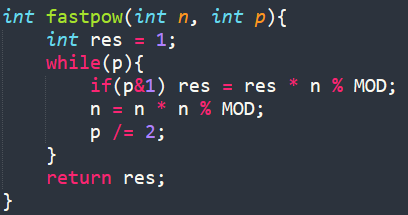
\includegraphics[]{images/code8.png}
    \end{center}
\end{frame}

\begin{frame}{練習題} 
    \begin{block}{CSES - Exponentiation}
        給你兩個數字 $a,b$,請輸出 $a^b \bmod 10^9+7$ 的答案。
    \end{block}
\end{frame}

\section{數論}

\begin{frame}{什麼是數論?}
    \begin{itemize}
        \item 數論是數學的其中一個分支,主要研究整數的性質
        \item 整數、質數、模運算等等的都是數論的範圍
    \end{itemize}
\end{frame}

\begin{frame}{質因數分解}
    \begin{itemize}
        \item 首先,我們先從大家最熟悉的東西開始談,也就是質因數分解
        \item 他的方式有很多,而我們先從最簡單的方式開始談談
    \end{itemize}
\end{frame}

\begin{frame}[fragile]{質因數分解}
    \begin{itemize}
        \item 首先,既然我們想要質因數分解一個數字 $n$,則我們可以從 $2$ 開始一路跑到 $n$
        \item 如果找到 $n$ 的因數時,就一直將他除掉,最後得到的那些數字就會是 $n$ 的因數了。
        \item 時間複雜度:$O(n)$
    \end{itemize}
    \begin{center}
        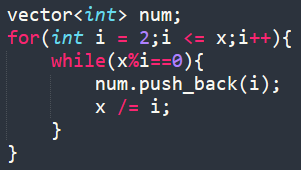
\includegraphics[]{images/code1.png}
    \end{center}
\end{frame}

\begin{frame}[fragile]{質因數分解}
    \begin{itemize}
        \item<1-> 不過,我們真的需要跑到 $n$ 那麼多個數字嗎? \pause
        \item<2-> 其實不用,我們會發現對於 $n$,如果他不是質數,他的質因數的大小不會超過 $\sqrt{n}$  \pause
        \item<3-> 因此,其實我們只要從 $2$ 枚舉到 $\sqrt{n}$ 就可以將這個數字質因數完了
        \item<3-> 時間複雜度: $O(\sqrt{n})$
    \end{itemize} 
    \begin{center}
        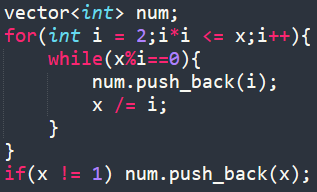
\includegraphics[]{images/code2.png}
    \end{center}
\end{frame}

\begin{frame}{質因數分解}
    \begin{itemize}
        \item<1-> 這個方式聽起來已經很快了吧! 
        \item<1-> 不過如果 $n$ 很小,我們有更快的方式可以處理這件事!
        \item<2-> 而這個方式就是預處理! 首先,我們要先知道怎麼找 $1 \sim n$ 之間的所有質數。
    \end{itemize} 
\end{frame}

\begin{frame}{判斷質數}
    \begin{itemize}
        \item<1-> 我們要如何判斷 $1 \sim n$ 哪些數字會是質數呢?
        \item<2-> 假設我們已經知道 $x$ 是質數了,那我們可以知道 $2x, 3x, \ldots$ 就都不會是質數了
        \item<3-> 我們可以預先將所有數字都先設質數,然後用上面的方法跑過每個數字和他們的倍數
        \item<4-> 這個方法叫做「埃氏篩法 (Sieve of Eratosthenes)」
    \end{itemize}
\end{frame}

\begin{frame}[fragile]{判斷質數}
    \begin{center}
        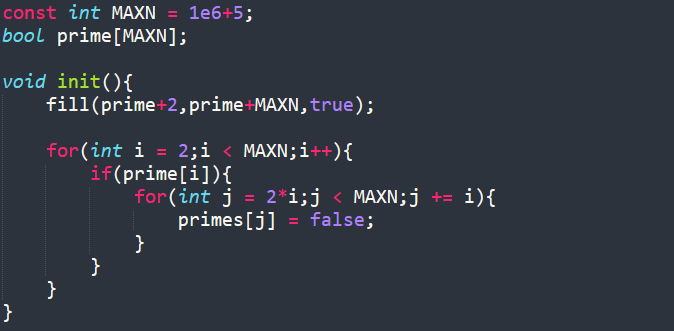
\includegraphics[scale=0.75]{images/code4.png}
    \end{center}
\end{frame}

\begin{frame}[fragile]{判斷質數}
    \begin{itemize}
        \item<1-> 不過這個方式的時間複雜度是多少呢?
        \item<1-> $\displaystyle O(\frac{n}{2} + \frac{n}{3} + \frac{n}{5} + \cdots) \approx O(n \log \log n)$
        \item<2-> 有興趣的人可以去查查看為什麼他會是這個複雜度,可以使用泰勒級數等方式證明
    \end{itemize}
\end{frame}

\begin{frame}[fragile]{判斷質數}
    題外話: 剛剛提到了埃氏篩法的神奇複雜度估算,我們在枚舉因數時會使用到以下程式碼
    \begin{center}
        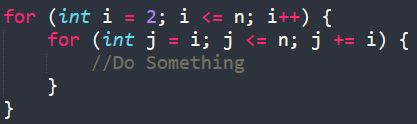
\includegraphics[]{images/code10.png}
    \end{center} \pause
    複雜度會是 $\displaystyle O(\frac{n}{1}+\frac{n}{2}+\dots)$,用積分 $\displaystyle \int^n_1 \frac{1}{x} dx = \ln(n)$ 的方式來估計會是 $O(n \log n)$ \\
    有人會稱這個東西為 Harmonic Series (調和級數) 的複雜度,總之就是一個小技巧
\end{frame}

\begin{frame}[fragile]{判斷質數}
    \begin{itemize}
        \item<1-> 雖然剛剛那個方式已經非常快速了,大部分的問題也都可以直接解決
        \item<1-> 不過事實上還有更快的作法可以幫助我們做到這件事
        \item<3-> 我們來看看下面這份 code
    \end{itemize}
\end{frame}

\begin{frame}[fragile]{判斷質數}
    \begin{center}
        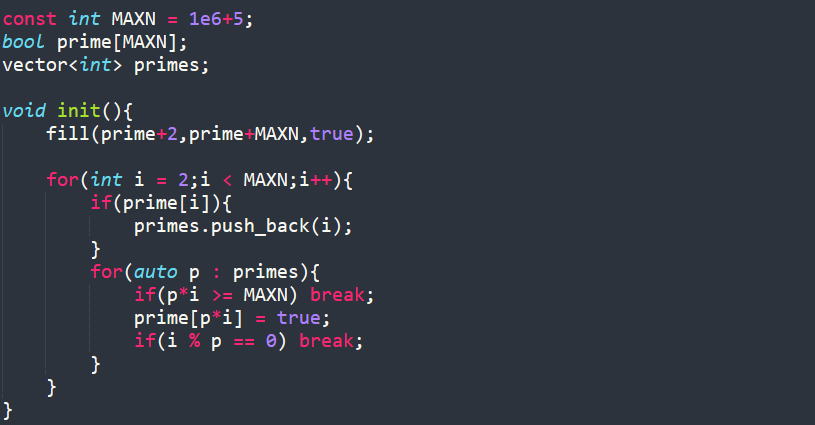
\includegraphics[scale=0.6]{images/code5.png}
    \end{center}
\end{frame}

\begin{frame}[fragile]{判斷質數}
    \begin{itemize}
        \item<1-> 這份 code 的時間複雜度是$O(n)$ ,也就是線性的
        \item<2-> 我們通常稱這個做法為「線性篩」
        \item<3-> 有了上面這兩個篩法,我們就可以來做質因數分解了!
    \end{itemize}
\end{frame}

\begin{frame}{回到質因數分解}
    \begin{itemize}
        \item<1-> 首先,要進行更快的質因數分解,我們要對每個人找他們的 LPF
        \item<2-> 我們可以使用剛剛的兩個篩法進行預處理
        \item<2-> 就可以在 $O(\log n)$ 的時間對 $n$ 進行質因數分解了!
    \end{itemize}
    \begin{alertblock}{Lowest Prime Factor (最小質因數)}
        對於一個數字 $x$,我們定義他的 \texttt{lpf[x]} 為他最小的質因數 \\
        \vspace{5mm}
        範例: \texttt{lpf[2]} = $2$、\texttt{lpf[15]} = $3$
    \end{alertblock}
\end{frame}

\begin{frame}{回到質因數分解}
    \begin{itemize}
        \item<1-> 首先,要進行更快的質因數分解,我們要對每個人找他們的 LPF
        \item<2-> 我們可以使用剛剛的兩個篩法進行預處理
        \item<2-> 就可以在 $O(\log n)$ 的時間對 $n$ 進行質因數分解了!
    \end{itemize}
    \begin{alertblock}{Lowest Prime Factor (最小質因數)}
        對於一個數字 $x$,我們定義他的 \texttt{lpf[x]} 為他最小的質因數 \\
        \vspace{5mm}
        範例: \texttt{lpf[2]} = $2$、\texttt{lpf[15]} = $3$
    \end{alertblock}
\end{frame}

\begin{frame}{回到質因數分解}
    附上有 lpf 之後的質因數分解 code
    \begin{center}
        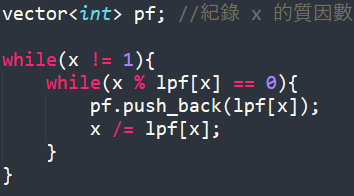
\includegraphics[]{images/code11.png}
    \end{center}
\end{frame}

\begin{frame}{例題}
    \begin{block}{Ten Point Round \#22 pI - 狐狸買氣球 (Balloon)}
        現在你有一個長度為 $n$ 的序列 $a_1, a_2, \dots, a_n$,定義一個數字 $x$ 的美麗程度為將 $x$ 寫成 $x = p_1^{b_1} p_2^{b_2} \ldots p_k^{b_k}$ 後,$\sum\limits_{i=1}^k (p_i \times b_i)$ 的數值。現在有 $q$ 筆詢問,每筆詢問請輸出區間 $[l,r]$ 所有數字相乘後的美麗程度為何? \\
        \vspace{5mm}
        測資範圍: 
        \begin{itemize}
            \item $1 \le n,q \le 10^6$
            \item $1 \le a_i \le 2 \times 10^6$
        \end{itemize}
    \end{block}
    \begin{itemize}
        \item<1-> 這題一樣留點時間給大家想想
    \end{itemize}
\end{frame}

\begin{frame}{例題}
    \begin{block}{Ten Point Round \#22 pI - 狐狸買氣球 (Balloon)}
        現在你有一個長度為 $n$ 的序列 $a_1, a_2, \dots, a_n$,定義一個數字 $x$ 的美麗程度為將 $x$ 寫成 $x = p_1^{b_1} p_2^{b_2} \ldots p_k^{b_k}$ 後,$\sum\limits_{i=1}^k (p_i \times b_i)$ 的數值。現在有 $q$ 筆詢問,每筆詢問請輸出區間 $[l,r]$ 所有數字相乘後的美麗程度為何? \\
        \vspace{5mm}
        測資範圍: 
        \begin{itemize}
            \item $1 \le n,q \le 10^6$
            \item $1 \le a_i \le 2 \times 10^6$
        \end{itemize}
    \end{block}
    \begin{itemize}
        \item 應該會發現,不同的數字其實貢獻可以分別討論
        \item 然後我們可以依序對每個 $a_i$ 進行質因數分解
        \item 這樣的複雜度會是 $O(n \log C)$ ($C$ 是 $a_i$ 的值域)
        \item 接著使用前綴和就可以 $O(1)$ 詢問了
    \end{itemize}
\end{frame}

\begin{frame}{練習題}
    \begin{block}{CSES - Counting Divisors}
        給你一個數字 $x$,請輸出 $x$ 有幾個因數。\\
        \vspace{5mm}
        提示: 若 $n=p_1^{\alpha_1} p_2^{\alpha_2} \dots p_k^{\alpha_k}$,則 $n$ 有 $\prod_{i=1}^k (\alpha_i+1)$ 個因數
    \end{block}
    \begin{block}{Zerojudge a010. 因數分解}
        給你一個數字 $x$,請對 $x$ 質因數分解。
    \end{block}
    \begin{block}{CSES - Common Divisors}
        你有 $n$ 個數字,你希望能找到在這個陣列中尋找兩個數字時,他們的最大公因數最大可能是多少?\\
        \vspace{5mm}
        提示: 調和級數 $O(n \log n)$
    \end{block}
\end{frame}

\begin{frame}{最大公因數 (Greatest Common Divisor)}
     \begin{itemize}
         \item<1-> 接著,我們來談談最大公因數
         \item<2-> 相信很多人都知道 C++ 其實有內建 \texttt{\_\_gcd(x,y)} 這個函數可以找 $x,y$ 的最大公因數
         \item<2-> 而 C++17 之後,甚至可以直接使用 \texttt{gcd(x,y)} 與 \texttt{lcm(x,y)}
         \item<3-> 不過在此,我們還是來談談計算最大公因數的方式
     \end{itemize}
\end{frame}

\begin{frame}{最大公因數 (Greatest Common Divisor)}
     \begin{itemize}
         \item<1-> 要計算最大公因數,我們最常使用的方式就是所謂的「輾轉相除法 (Euclidean Algorithm)」
         \item<1-> 或者說他是「歐幾里得演算法」,這個方法相信大家在國小或國中時就已經學過了
     \end{itemize}
\end{frame}

\begin{frame}{最大公因數 (Greatest Common Divisor)}
    \begin{alertblock}{輾轉相除法 (歐幾里得演算法)}
        當我們有兩個數字時,我們可以利用 $\gcd(a,b) = \gcd(b,a \bmod b)$ 的想法,持續向下遞迴,直到我們得到 $\gcd(x,0)$ 時,$x$ 即為 $\gcd(a,b)$
    \end{alertblock} 
    \begin{itemize}
        \item 此算法的時間複雜度最差為 $O(\log \max(a,b))$,在 $a,b$ 為費氏數時會有 worst case
        \item 不過在一般的情況下,他基本上會跑得非常快速。
    \end{itemize}
\end{frame}

\begin{frame}{最大公因數 (Greatest Common Divisor)}
    \begin{alertblock}{輾轉相除法 (歐幾里得演算法)}
        當我們有兩個數字時,我們可以利用 $\gcd(a,b) = \gcd(b,a \bmod b)$ 的想法,持續向下遞迴,直到我們得到 $\gcd(x,0)$ 時,$x$ 即為 $\gcd(a,b)$
    \end{alertblock} 
    \begin{center}
        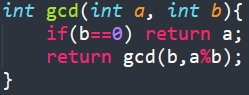
\includegraphics[]{images/code6.png}
    \end{center}
\end{frame}

\begin{frame}{貝祖定理 (Bézout's identity))}
    \begin{alertblock}{貝祖定理 (Bézout's identity)}
        對於任何整數 $a,b,c$,若 $ax+by = c$ 存在整數解 $\iff$ $gcd(a,b) | c$
    \end{alertblock} 
\end{frame}

\begin{frame}{貝祖定理 (Bézout's identity)}
    \begin{block}{證明}
        \begin{itemize}
            \item $(\Rightarrow)$ 
            假設 $ax+by=c$ 存在整數解 $x=x_0, y=y_0$,則 $ax_0+by_0=c$,由於 $gcd(a,b) | a, \ gcd(a,b) | b$,原式可寫為 $gcd(a,b) (\dfrac{a}{gcd(a,b)}x_0 + \dfrac{b}{gcd(a,b)}y_0) = c$,故 $gcd(a,b) | c$
            \item $(\Leftarrow)$ 假設 $a=0$,則 $gcd(a,b)=b$,式子變為 $by = c$,若 $x,y$ 存在整數解,則 $b|c$。 
            \newline
            假設 $a,b$ 皆不為 $0$,設集合 $S = \{ax+by|x,y \in \mathbb{Z}^2\}$,而 $S \cap \mathbb{N}$ 並非空集合 (必存在 $|a|, |b|$)。根據良序定理,$S$ 內必存在一個最小的正整數 $d = ax_0+by_0$。考慮 $S$ 中另一個數字 $p=ax_1+by_1$。根據除法原理,$p = qd + r$,其中 $q \in \mathbb{Z}, \ 0 \le r < d$。因此 $r = p-qd = (ax_1+by_1)-q(ax_0+by_0) = a(x_1-qx_0)+b(y_1-qy_0)$,得 $r \in S$。又因為前面的假設,$r$ 必為 $0$。任何 $S$ 當中的數字皆為 $d$ 的倍數。而 $a,b \in S$,因此 $d|a, \ d|b \Rightarrow d|gcd(a,b)$。而 $ax+by=d$ 有整數解,因此 $ax+by=gcd(a,b)$ 必有整數解。又因為 $gcd(a,b)|c$,因此 $ax+by=c$ 必有整數解
        \end{itemize}
    \end{block}
\end{frame}

\begin{frame}{拓展歐幾里得演算法 (Extended GCD Algorithm)}
    有了剛剛的貝祖定理之後,如果 $ax+by=c$ 有整數解,我們要怎麼找到一組 $x,y$ 呢?
    \begin{alertblock}{拓展歐幾里得演算法 (Extended GCD Algorithm)}
        如果 $ax+by=c$ 有整數解,則 $bx'+(a \bmod b)y' = c$ 必有整數解 ($\gcd$ 不變),我們將 $a \bmod b$ 轉換為 $a - b \Big \lfloor \dfrac{a}{b} \Big \rfloor$。原式可以轉換為 
        $$bx' + (a - b \Big \lfloor \dfrac{a}{b} \Big \rfloor)y' = c$$
        $$bx' + ay' - b \Big \lfloor \dfrac{a}{b} \Big \rfloor y' = c$$
        $$ay' + b (x' - \Big \lfloor \dfrac{a}{b} \Big \rfloor y') = c$$
        我們可以使用遞迴的方式一路由下往上計算答案
    \end{alertblock} 
\end{frame}

\begin{frame}{拓展歐幾里得演算法 (Extended GCD Algorithm)}
    以下為範例程式碼
    \begin{center}
        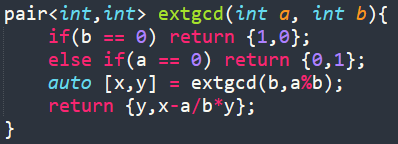
\includegraphics[]{images/code7.png}
    \end{center}
\end{frame}

\begin{frame}{練習題}
    \begin{block}{NHDK Ten Point Round \#21 - 調色盤}
        你有 $n$ 個數字 $a_1, \ldots, a_n$,接著有 $q$ 筆詢問,每次問你是否存在一組整數解 $\{b_1,\ldots,b_n\}$ 可以使得 $a_1b_1 + a_2b_2 + \dots + a_nb_n + 1115 = T$。
    \end{block}
    \begin{block}{Atcoder Beginner Contest 186 pE - Throne}
        有 $n$ 個椅子排成環狀,這 $n$ 個椅子其中有一個是王位,目前 Colten 坐在離王位順時鐘 $s$ 格的椅子上,他每一次移動會順時鐘移動到 $k$ 格後的椅子上,請問他至少要幾次移動才能坐到王位上,或者永遠坐不到。
    \end{block}
\end{frame}

\begin{frame}{同餘 (Modular Congruence)}
    在我們講什麼是同餘之前,我們要先介紹「模運算 (Modular arithmetic)」,通常在題目會遇到要輸出答案 $\bmod \ 10^9+7$ 或 $998244353$ 的題目時,會用到這個運算
    \begin{alertblock}{模運算}
        \begin{enumerate}
            \item 基本上就是對整數除法取餘數,也就是大家熟悉程式中的的 \texttt{\%}
            \item $r = x \bmod m$,我們可以將 $x$ 寫成 $x = km + r, \ 0 \le r < m$ 
            \item $m \mid x \iff x \bmod m = 0$,表示存在一個 $n$ 可以使得 $x = mn$
        \end{enumerate}
    \end{alertblock}
\end{frame}

\begin{frame}{同餘 (Modular Congruence)}
    而當我們在同一個模數底下做運算時,我們會用到同餘這個概念
    \begin{alertblock}{同餘 (Modular Congruence)}
        \begin{enumerate}
            \item $a \equiv b \pmod m$ 表示 $a \bmod m = b \bmod m$ 或 $(a-b) \bmod m = 0$
            \item 如果 $a \equiv b \pmod m$,則
                \begin{itemize}
                    \item $a+c \equiv b+c \pmod m$
                    \item $a-c \equiv b-c \pmod m$
                    \item $ac \equiv bc \pmod m$
                    \item 不滿足 $a \div c \equiv b \div c \pmod m$
                \end{itemize}
            \item 如果 $a \equiv b \pmod m, \ p \equiv q \pmod m$
            \begin{itemize}
                \item $a+p \equiv b+q \pmod m$
                \item $ap \equiv bq \pmod m$
            \end{itemize}
        \end{enumerate}
    \end{alertblock}
\end{frame}

\begin{frame}{同餘 (Modular Congruence)}
    而我們來證明一下剛剛的那幾個性質吧  
    \begin{block}{加法的證明 ($a+c \equiv b+c \pmod m$)}
        當 $a \equiv b \pmod m$ 時,假設 $a=k_1m + r, \ b = k_2m + r, \ k_1, k_2, r \in \mathbb{Z}$ \\
        \vspace{5mm}
        則 $a+c = k_1m+r+c, \ b+c = k_2m + r + c \Rightarrow (a+c)-(b+c) = (k_1-k_2)m \Rightarrow (a+c)-(b+c) \bmod m = 0$,因此 $a+c \equiv b+c \pmod m$
    \end{block}
\end{frame}

\begin{frame}{同餘 (Modular Congruence)}
    \begin{block}{減法的證明 ($a-c \equiv b-c \pmod m$)}
        當 $a \equiv b \pmod m$ 時,假設 $a=k_1m + r, \ b = k_2m + r, \ k_1, k_2, r \in \mathbb{Z}$ \\
        \vspace{5mm}
        則 $a-c = k_1m+r-c, \ b-c = k_2m + r - c \Rightarrow (a+c)-(b+c) = (k_1-k_2)m \Rightarrow (a-c)-(b-c) \bmod m = 0$,因此 $a-c \equiv b-c \pmod m$
    \end{block}
\end{frame}

\begin{frame}{同餘 (Modular Congruence)}
    \begin{block}{乘法的證明 ($ac \equiv bc \pmod m$)}
        當 $a \equiv b \pmod m$ 時,假設 $a=k_1m + r, \ b = k_2m + r, \ k_1, k_2, r \in \mathbb{Z}$ \\
        \vspace{5mm}
        則 $ac = (k_1m+r)c, \ bc = (k_2m + r)c \Rightarrow ac-bc = (k_1-k_2)cm \Rightarrow ac-bc \bmod m = 0$,因此 $a-c \equiv b-c \pmod m$
    \end{block}
\end{frame}

\begin{frame}{同餘 (Modular Congruence)}
    \begin{itemize}
        \item 既然我們剛剛講到了加減乘,那要進行除法怎麼辦呢?
        \item 模運算並不滿足直接進行除法運算的性質,那我們該怎麼處理呢?
        \item 事實上,在有模數的運算系統下,有另外一個東西可以幫助我們做除法的操作
    \end{itemize}
\end{frame}

\begin{frame}{同餘 (Modular Congruence)}
    \begin{alertblock}{模反元素 (Modular Inverse)}
        對於一個元素 $x$,在 $\bmod \ m$ 的系統下,$x^{-1}$ 為滿足 $xx^{-1}\equiv 1 \pmod m$ 的數字,我們稱 $x^{-1}$ 為 $x$ 的「模反元素」或「模逆元」。而並不是對於所有 $x$ 皆存在一個模反元素,若模反元素存在則 $x$ 必與 $m$ 互質。
    \end{alertblock}
    \begin{itemize}
        \item<2-> 因此,當我們在模運算系統下要計算除法時,會使用 $ab^{-1}$ 表示 $a$ 除以 $b$ 的操作
        \item<3-> 不過,我們要怎麼計算這個數字呢?
        \item<4-> 主流的方式有三種,我們來一一介紹
    \end{itemize}
\end{frame}

\begin{frame}{模反元素找法}
    \begin{itemize}
        \item 費馬小定理 (只有在 $m$ 是質數時可以使用)
        \item 建表法 (只有在 $m$ 是質數時可以使用)
        \item 拓展歐幾里得定理 (又稱 extgcd,當 $gcd(a,m) = 1$ 時可以使用)
    \end{itemize}
\end{frame}

\begin{frame}{模反元素找法一 - 費馬小定理 (Fermat's Little Theorem)}
    \begin{alertblock}{費馬小定理 (Fermat's Little Theorem)}
        當 $p$ 是質數時,對於任一個整數 $a$,滿足 $a^{p-1} \equiv 1 \pmod p$
    \end{alertblock}
\end{frame}

\begin{frame}{模反元素找法一 - 費馬小定理 (Fermat's Little Theorem)}
    \begin{alertblock}{費馬小定理 (Fermat's Little Theorem)}
        當 $p$ 是質數時,對於任一個整數 $a$,滿足 $a^{p-1} \equiv 1 \pmod p$
    \end{alertblock}
    \begin{block}{證明}
        \begin{enumerate}
            \item 當 $p|a$ 時,必滿足 $a^p \equiv a \pmod p$。
            \item 對於 $a,2a,\ldots,(p-1)a$,這些數字除以 $p$ 的餘數必一一對應到 $1,2,\ldots,p-1$,否則任意兩個相同餘數的數字可以相減使得 $a|p$。因此 $(p-1)!a^{p-1} \equiv a \times 2a \times \cdots \times (p-1)a \equiv (p-1)! \pmod p$。得 $a^{p-1}\equiv 1 \pmod p$
        \end{enumerate}
    \end{block}
\end{frame}

\begin{frame}{模反元素找法一 - 費馬小定理 (Fermat's Little Theorem)}
    \begin{alertblock}{費馬小定理 (Fermat's Little Theorem)}
        當 $p$ 是質數時,對於任一個整數 $a$,滿足 $a^{p-1} \equiv 1 \pmod p$
    \end{alertblock}
    要使用這個定理計算模反元素的話,我們可以將原式兩邊同乘以 $a^{-1}$,得到 
    $$a^{p-2} \equiv a^{-1} \pmod p$$
    因此,我們可以使用快速冪來得到 $a^{-1}$。\\
    時間複雜度: $O(\log p)$
\end{frame}

\begin{frame}{模反元素找法二 - 建表法}
    假設我們想要計算 $i$ 在 $\mod \ p$ ($p$ 必須是質數) 下的模反元素,推導過程如下
    \begin{align*}
        p - i \times \Big \lfloor \dfrac{p}{i} \Big \rfloor&= p \bmod i \\
        p - i \times \Big \lfloor \dfrac{p}{i} \Big \rfloor &\equiv p \bmod i \pmod p \\
        p \times i - i \times \Big \lfloor \dfrac{p}{i} \Big \rfloor &\equiv p \bmod i \pmod p \\
        i(p - \Big \lfloor \dfrac{p}{i} \Big \rfloor)(p \bmod i)^{-1} &\equiv 1 \pmod p \\
        (p - \Big \lfloor \dfrac{p}{i} \Big \rfloor)(p \bmod i)^{-1} &\equiv i^{-1} \pmod p 
    \end{align*}
    這個方式可以讓我們用遞迴的方式往下做,雖然個人不確定複雜度上界究竟是多少,但經過測試,幾乎都能在 $O(\log p)$ 的時間計算完,而我們可以使用一個迴圈依序計算每個數字的模反元素,複雜度 $O(p)$。
\end{frame}

\begin{frame}{模反元素找法二 - 建表法}
    參考程式碼
    \begin{center}
        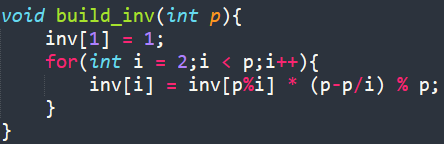
\includegraphics[]{images/code9.png}
    \end{center}
\end{frame}

\begin{frame}{模反元素找法三 - 拓展歐幾里得定理 (Extended GCD)}
    當我們要找 $a$ 在 $\bmod \ m$ 下的模反元素,若滿足 $gcd(a,m)=1$,則我們可以列出
    $$aa^{-1} + bm = 1$$
    使用拓展歐幾里得找 $a^{-1}$ 即可
\end{frame}

\begin{frame}{歐拉函數 (Euler Phi Function)}
    \begin{alertblock}{歐拉函數 (Euler Phi Function)}
        對於正整數 $n$,定義 $\phi(n)$ 為小於等於 $n$ 且與 $n$ 互質的正整數數量。
        \begin{enumerate}
            \item 對於一個質數 $p$,$\phi(p) = p-1$
            \item 若 $a,b$ 互質,則 $\phi(ab) = \phi(a) \phi(b)$ (積性函數)
            \item $a^{\phi(p)} \equiv 1 \pmod p$ (歐拉定理)
            \item 假設 $n=p_1^{\alpha_1}p_2^{\alpha_2}\dots p_k^{\alpha_k}$,則 $\phi(n) = n \prod_{i=1}^k (1-\frac{1}{p_i})$
        \end{enumerate}
    \end{alertblock}
\end{frame}

\begin{frame}{中國剩餘定理 (Chinese Remainder Theorem)}
    在孫子算經中,有一題「物不知數」,題目如下:
    \begin{center}
        「有物不知其數,三三數之剩二,五五數之剩三,七七數之剩二。問物幾何?」
    \end{center}
\end{frame}

\begin{frame}{中國剩餘定理 (Chinese Remainder Theorem)}
    寫成數學式會長這樣
    \begin{equation*}
        \quad \left\{ \begin{matrix} x \equiv 2 \pmod {3} \\ x \equiv 3 \pmod {5} \\ x \equiv 2 \pmod {7} \end{matrix} \right.
    \end{equation*} \pause
    這個問題其實大家在國中課本可能也有看過類似的題目,像韓信點兵等等的問題。 \\
    而如何找到這個問題的解,就是我們要來解決的。
\end{frame}

\begin{frame}{中國剩餘定理 (Chinese Remainder Theorem)}
    題外話,上面那題的解,在孫子算經中同樣也有描述
    \begin{center}
        「三人同行七十希,五樹梅花廿一支,七子團圓正半月,除百零五便得知」
    \end{center}
    也就是說,將除以三的餘數乘以 $70$,除以五的餘數乘以 $21$,除以七的餘數乘以 $15$,接著除以 $105$ 的餘數就會是答案了! \\
    $$2 \times 70 + 3 \times 21 + 2 \times 15 \equiv 233 \equiv 23 \pmod {105}$$
\end{frame}

\begin{frame}{中國剩餘定理 (Chinese Remainder Theorem)}
    因此,中國剩餘定理就是一個可以幫助我們解決一元一次同餘聯立方程式的方法
    \begin{equation*}
        \quad \left\{ \begin{matrix} x \equiv a_1 \pmod {m_1} \\ x \equiv a_2 \pmod {m_2} \\ x \equiv a_3 \pmod {m_3} \\ \vdots \\ x \equiv a_n \pmod {m_n} \end{matrix} \right.
    \end{equation*}
\end{frame}

\begin{frame}{中國剩餘定理 (Chinese Remainder Theorem)}
    這個問題有兩種解法:
    \begin{enumerate}
        \item 使用通解的形式找到答案 (數學上常用的方式)
        \item 使用拓展歐幾里得算法計算答案 (比賽中常用的方式)
    \end{enumerate}
    第一種作法的話,我們會快速帶過,在競程上比較常使用第二種方式
\end{frame}

\begin{frame}{中國剩餘定理 (Chinese Remainder Theorem)}
    \begin{alertblock}{構造通解的方式}
        假設 $m_1, m_2, \dots, m_n$ 
        \begin{enumerate}
            \item 設 $M = m_1 m_2 \dots m_n = \prod_{i=1}^n m_i$,而 $M_i = M/m_i$
            \item 設 $t_i = M^{-1}$,意即 $t_i$ 是 $M_i$ 的模反元素  
            \item 則通解會是 $x \equiv a_1t_1M_1 + a_2t_2M_2 + \dots + a_n t_n M_n \equiv \sum_{i=1}^n a_i t_i M_i \pmod M$
        \end{enumerate}
    \end{alertblock}
\end{frame}

\begin{frame}{中國剩餘定理 (Chinese Remainder Theorem)}
    \begin{alertblock}{使用拓展歐幾里得的方法}
        先假設我們只想要找兩個式子的解 ($m_1, m_2$ 可以不互質)
        $$\quad \left\{ \begin{matrix} x \equiv a_1 \pmod {m_1} \\ x \equiv a_2 \pmod {m_2} \end{matrix} \right.$$
        則我們可以知道對於兩個整數 $k_1, k_2$
        $$\quad \left\{ \begin{matrix} x = k_1m_1 + a_1 \\ x = k_2m_2 + a_2 \end{matrix} \right.$$
        合併兩個式子,我們會得到
        $$k_1m_1 + a_1 = k_2m_2 + a_2$$
        移項一下會得到
        $$m_1k_1 - m_2k_2 = a_2-a_1$$
    \end{alertblock}
\end{frame}

\begin{frame}{中國剩餘定理 (Chinese Remainder Theorem)}
    \begin{alertblock}{使用拓展歐幾里得的方法}
        接著我們可以使用 extgcd,找到一組 $k_1, k_2$ 的解 $(k_1', k_2')$ \\
        \vspace{5mm}
        再將 $k_1$ 代入 $x = a_1 + m_1k_1$ 的式子當中,兩式就合併成 
        $$x \equiv a_1 + m_1 k_1 \pmod {lcm(m_1,m_2)}$$
    \end{alertblock}
\end{frame}

\begin{frame}{例題}
    \begin{block}{CSES - Exponentiation II}
        給你三個數字 $a,b,c$,請輸出 $a^{b^c} \bmod 10^9+7$ 的值 
    \end{block}
    \begin{itemize}
        \item<1-> 看到這題,我們可以直接使用上面的兩種方法去簡化這題
        \item<1-> 可以使用歐拉函數或費馬小定理去做化簡
        \item<2-> $a^{b^c} \equiv a^{b^c \bmod 10^9+5} \pmod{10^9+7}$
    \end{itemize}
\end{frame}

\begin{frame}{練習題}
    \begin{block}{Codeforces 907F - Power Tower}
        你有 $n$ 個數字 $a_1,a_2,\ldots,a_n$,和一個模數 $m$,接著有 $q$ 筆詢問,每次詢問區間 $[l,r]$ 的
        $$a_l^{a_{l+1}^{\ldots^{a_r}}} \bmod m$$
    \end{block}
    
    \begin{block}{Kattis - Chinese Remainder Theorem}
        實作中國剩餘定理,模數不一定互質
    \end{block}
\end{frame}

\section{組合計數}

\begin{frame}{加法原理 (Addition Rule)}
    \begin{alertblock}{加法原理 (Addition Rule)}
        若一個集合 $S$ 可以被分成 $k$ 個互斥的集合 $S_1, S_2, \dots, S_k$,則 $$|S| = |S_1|+|S_2|+\dots+|S_k|$$
    \end{alertblock} \pause
    簡單來說,一個大問題,我們可以想成許多個互不相干的問題,將這些問題的答案相加就會是總共的方案數了。
\end{frame}

\begin{frame}{加法原理 (Addition Rule)}
    假設從狀態 $1$ 到狀態 $2$ 有 $3$ 種 $A$ 方案,$2$ 種 $B$ 方案,$1$ 種 $C$ 方案,則一共有 $6$ 種方案
    \begin{center}
        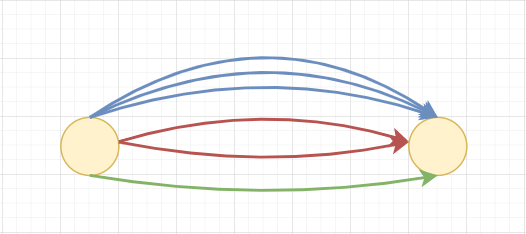
\includegraphics[scale=0.75]{images/addition.png}
    \end{center}
\end{frame}

\begin{frame}{乘法原理 (Multiplication Rule)}
    \begin{alertblock}{乘法原理 (Multiplication Rule)}
        若一個方案 $S$ 可以被拆成 $k$ 個步驟,而第 $i$ 個步驟 $S_i$ 共有 $|S_i|$ 種方案數,則
        $$|S| = |S_1| \cdot |S_2| \cdot \dots \cdot |S_k|$$
    \end{alertblock} \pause
    簡單來說,一個大問題,如果他有很多個不同的步驟,則這些方案數相乘就會是總共的方案數了
\end{frame}

\begin{frame}{乘法原理 (Multiplication Rule)}
    假設從狀態 $1$ 走到 $2$ 有 $2$ 種方案,從 $2$ 走到 $3$ 有 $3$ 種方案,則一共有 $6$ 種方案從 $1$ 到 $3$
    \begin{center}
        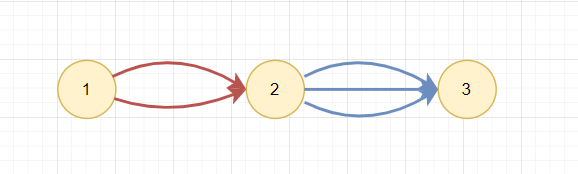
\includegraphics[scale=0.75]{images/multiplication.png}
    \end{center}
\end{frame}


\begin{frame}{排列 (Permutation)}
    對於相異的元素,計算他們經由不同順序可以組成的排列數量。
    \begin{alertblock}{排列 (Permutation)}
        有 $n$ 個相異元素時,總共有 $n!$ 種不同的排列。 
        \begin{itemize}
            \item $n! = 1 \times 2 \times \dots \times n$
            \item $0! = 1$
        \end{itemize}
    \end{alertblock}
\end{frame}

\begin{frame}{排列 (Permutation)}
    以下為 $\{a,b,c\}$ 的 $3! = 6$ 種排列方式
    \begin{center}
        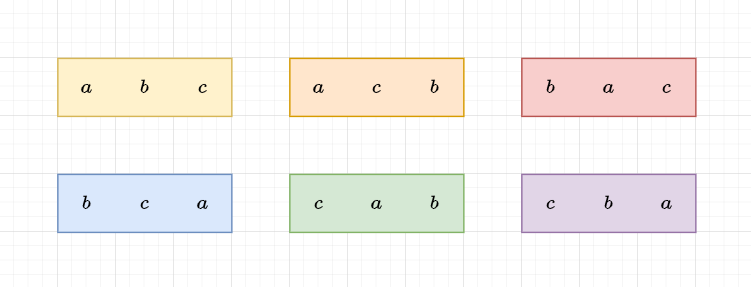
\includegraphics[width=\textwidth]{images/permutation.png}
    \end{center}
\end{frame}

\begin{frame}{排列 (Permutation)}
    \begin{alertblock}{排列 (Permutation)}
        從 $n$ 個相異元素選出 $r$ 個做排列時,總共有 $P^n_r$ 種不同的排列。 
        \begin{itemize}
            \item $P^n_r = \dfrac{n!}{(n-r)!}$
        \end{itemize}
    \end{alertblock}
\end{frame}

\begin{frame}{排列 (Permutation)}
    以下從 $\{a,b,c\}$ 中取出 $2$ 個元素做排列時的 $P^3_2 = 6$ 種排列方式
    \begin{center}
        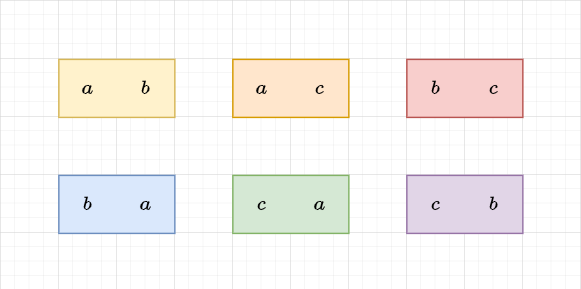
\includegraphics[scale=0.75]{images/nPr.png}
    \end{center}
\end{frame}

\begin{frame}{排列 (Permutation)}
    \begin{alertblock}{不盡相異物排列}
        有 $n$ 個元素,而每個元素的出現次數共有 $m_i$ 次,則排列的次數一共有
        $$\dfrac{n!}{m_1!m_2!\dots m_k!}$$
    \end{alertblock}
\end{frame}

\begin{frame}{例題}
    \begin{block}{CSES - Creating Strings II}
        給你一個字串 $s$,問你有幾個字串可以由 $s$ 經過重組後得到,由於數量可能很大,請輸出答案 $\bmod \ 10^9+7$。
    \end{block} \pause
    基本上就是套剛剛的公式而已,不過由於剛剛有除法以及取模操作,記得要使用模反元素,不能直接用除的!
\end{frame}

\begin{frame}{組合 (Combination)}
    \begin{alertblock}{組合 (Combination)}
        從 $n$ 個相異元素當中選出 $r$ 個元素的一共有 $C^n_r$ 種
        \begin{itemize}
            \item $C^n_r = \dfrac{n!}{(n-r)!r!}$
            \item $C^n_0 = 1$
            \item $C^n_r = C^n_{n-r}$
            \item $C^n_r$ 又可以被寫成 $\binom{n}{r}$
            \item $C^n_r = C^{n-1}_r + C^{n-1}_{r-1}$ (帕斯卡三角形)
        \end{itemize}
    \end{alertblock}
\end{frame}

\begin{frame}{組合 (Combination)}
    從 $\{a,b,c\}$ 當中任選 $2$ 個元素的方法,一共有 $C^3_2 = 3$ 種
    \begin{center}
        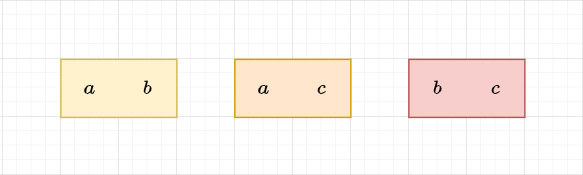
\includegraphics[width=\textwidth]{images/combination.png}
    \end{center}
\end{frame}

\begin{frame}{組合 (Combination)}
    從 $\{a,b,c\}$ 當中任選 $2$ 個元素的方法,一共有 $C^3_2 = 3$ 種
    \begin{center}
        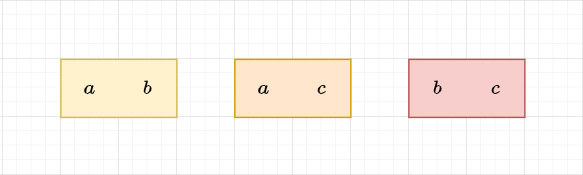
\includegraphics[width=\textwidth]{images/combination.png}
    \end{center}
\end{frame}

\begin{frame}{組合 (Combination)}
    \begin{alertblock}{重複組合 (Star and Bars)}
        從 $n$ 個元素中取出 $r$ 個,而這 $r$ 個元素可以重複出現,一共有 $H^n_r$ 種選法
        \begin{itemize}
            \item 等同於 $a_1+a_2+\dots+a_n = r$ 的非負整數解數量
            \item 英文稱為 Star and Bars,可以想成是 $r$ 個 $1$ 和 $n-1$ 個 $+$ 在做重複排列
            \item $H^n_r$ 又可以被寫成 $\displaystyle \left(\!\!{\binom {n}{r}}\!\!\right)$
            \item $H^n_r = C^{n+r-1}_{n-1}$ 
        \end{itemize}
    \end{alertblock}
\end{frame}

\begin{frame}{排容原理 (Inclusion-Exclusion Principle)}
    \begin{alertblock}{排容原理 (Inclusion-Exclusion Principle)}
        若我們有 $n$ 個集合 $A_1,A_2,\dots,A_n$,則
        $$\left|\bigcup^n_{i=1} A_i\right| = \sum_{1 \le i \le n} |A_i| - \sum_{1 \le i < j \le n} |A_i \cap A_j| + \dots + (-1)^{n+1} |A_1 \cap A_2 \cap \dots \cap A_n| $$
        \vspace{5mm}
        \begin{itemize}
            \item $n=2$ 時,有 $|A_1 \cup A_2| = |A_1| + |A_2| - |A_1 \cap A_2|$
            \item $n=3$ 時,有 $|A_1 \cup A_2 \cup A_3| = |A_1| + |A_2| + |A_3| - |A_1 \cap A_2| - |A_2 \cap A_3| - |A_3 \cap A_1| + |A_1 \cap A_2 \cap A_3|$
        \end{itemize}
    \end{alertblock}
\end{frame}

\begin{frame}{二項式定理 (Binomial Theorem)}
    \begin{alertblock}{二項式定理 (Binomial Theorem)}
        $$(1+x)^n = \binom{n}{0}x^0 + \binom{n}{1}x^1+ \dots + \binom{n}{n}x^n$$
    \end{alertblock}
\end{frame}

\begin{frame}{例題}
    \begin{block}{AtCoder Beginner Contest 178C - Ubiquity}
        請找到有多少個長度為 $N$ 的序列 $A_1,A_2,\dots,A_N$ 滿足
        \begin{itemize}
            \item 對於所有 $i$,$0 \le A_i \le 9$
            \item 至少存在一個 $i$ 使得 $A_i = 0$
            \item 至少存在一個 $i$ 使得 $A_i = 9$
        \end{itemize}
    \end{block} 
    \begin{itemize}
        \item 排容原理!
        \item 全部的數量 - (沒有 $0$) - (沒有 $9$) + (沒有 $0$ 也沒有 $9$)
        \item 答案就是 $10^n - 9^n - 9^n + 8^n$
    \end{itemize}
\end{frame}

\begin{frame}{例題}
    \begin{block}{CSES - Christmas Party}
        在一個聖誕節派對上,有 $n$ 個人在玩交換禮物,每個人都會送出一個禮物,也會收到一個禮物。請問有幾種送法可以讓這 $n$ 個人都收到不是自己送出去的禮物。
    \end{block}
    \begin{itemize}
        \item<1-> 這個問題其實是經典的「錯排」問題
        \item<2-> 我們可以用排容原理來思考看看
        \item<3-> 答案其實就是 全部 - (至少 $1$ 個人會收到自己的禮物) + (至少 $2$ 個人會收到自己的禮物) - (至少 $3$ 個人會收到自己的禮物) + $\ldots$
        \item<3-> $n! - \sum_{i=1}^n \binom{n}{i} (n-i)!$
    \end{itemize}
\end{frame}

\begin{frame}{例題}
    \begin{block}{Codeforces 453A - Little Pony and Expected Minimum}
        Colten 有一個 $m$ 面的均勻骰子,第 $i$ 面上有 $i$ 個點,接著他會骰這個骰子 $n$ 次。而他會將取這 $n$ 次骰出的最大值作為他的分數。請問他得到的分數期望值會是多少? \\
        \vspace{5mm}
        期望值的計算方式為 $\sum X_i \times P_i$
    \end{block} \pause
    \begin{itemize}
        \item<1-> 首先,我們會發現到每個價值的機率其實就是 $(\frac{1}{m})^n$
        \item<2-> 因此,我們只要能夠計算所有情況的價值總和即可
        \item<3-> 那我們要怎麼計算這個答案呢?
        \item<4-> 我們將最大值為 $x$ 的狀態分開思考
    \end{itemize}
\end{frame}

\begin{frame}{例題}
    \begin{block}{Codeforces 453A - Little Pony and Expected Minimum}
        Colten 有一個 $m$ 面的均勻骰子,第 $i$ 面上有 $i$ 個點,接著他會骰這個骰子 $n$ 次。而他會將取這 $n$ 次骰出的最大值作為他的分數。請問他得到的分數期望值會是多少? \\
        \vspace{5mm}
        期望值的計算方式為 $\sum X_i \times P_i$
    \end{block} \pause
    \begin{itemize}
        \item<1-> 假設 $n$ 次骰出來的最大值為 $x$,那總共有多少可能呢?
        \item<2-> 排容! 
        \item<3-> 答案其實就是 (其中一次骰出 $x$) - (其中兩次骰出 $x$) + (其中三次骰出 $x$) - \dots
        \item<4-> 不過其實有更簡單的方式! 
        \item<4-> 答案就是 全部 - (沒有骰出 $x$)
        \item<5-> 用一個迴圈跑過每種可能的 $x$ 即可
    \end{itemize}
\end{frame}

\begin{frame}{例題}
    \begin{block}{AtCoder Beginner Contest 178D - Redistribution}
        現在你有一個數字 $S$,請問有幾個不同的序列滿足其中所有的數字皆 $\ge 3$,且該序列的總和為 $S$
    \end{block} \pause
    \begin{itemize}
        \item 我們可以直接去枚舉序列的長度
        \item 接著套 $S-3$ 次的重複組合公式即可
    \end{itemize}
\end{frame}

\begin{frame}{例題}
    \begin{block}{Codeforces 1288C - Two Arrays}
        現在給你兩個數字 $n,m$,請找出總共有多少對的陣列 $(A,B)$ 滿足
        \begin{itemize}
            \item $A,B$ 的長度皆為 $m$
            \item $1 \le A_i, B_i \le n$
            \item 對於所有 $i$, $A_i \le B_i$
            \item $A$ 陣列是非遞減的 ($A_i \le A_{i+1}$)
            \item $B$ 陣列是非遞增的 ($B_i \ge B_{i+1}$)
        \end{itemize}
    \end{block} \pause
    \begin{itemize}
        \item<1-> 首先,我們觀察到 $A_n \le B_n$,而且 $A$ 是非遞減,$B$ 是非遞增的
        \item<2-> 如果我們知道 $A_i, B_i$ 會有哪些元素,則我們可以知道要怎麼分配這些數字
        \item<3-> $A_1,\dots,A_n,B_n,\dots,B_1$ 會是一個非遞減的陣列
        \item<4-> 我們可以發現 $1 \sim n$ 之間的數字總共出現的頻率會是 $2m$
        \item<5-> $f_1 + f_2 + \dots + f_n = 2m$ 的非負整數解數量!
    \end{itemize}
\end{frame}

\begin{frame}{例題}
    \begin{block}{Codeforces 893E - Counting Arrays}
        給你兩個數字 $x,y$,請找出有幾個整數陣列 $F$ 滿足
        \begin{itemize}
            \item $F$ 的長度為 $y$
            \item $\prod^y_{i=1} F_i = x$
        \end{itemize}
    \end{block} \pause
    \begin{itemize}
        \item 將不同的質因數分開思考,假設 $p$ 在 $x$ 的質因數分解中,次方一共是 $cnt_p$ 個
        \item 那我們可以把 $cnt_p$ 分配到 $y$ 個格子裡
        \item 直接使用重複組合的公式即可!
    \end{itemize}
\end{frame}

\begin{frame}{例題}
    \begin{block}{2020 臺北市資訊學科能力競賽 pC}
        總共有 $n$ 個格子,你可以在每一格上放上 $6$ 種棋子 (國王、皇后、騎士、主教、城堡、士兵) 其中之一,請問總共有幾種放法可以讓國王與皇后的出現次數皆為奇數。 \\
        \vspace{5mm}
        測資範圍: $n \le 10^9$
    \end{block} 
    \pause
    \begin{itemize}
        \item 這題實際上的作法是動態規劃 + 矩陣快速冪
        \item 不過前年在比賽中遇到這題時,被我用了數學解掉了
        \item 讓大家思考看看這題要怎麼處理
    \end{itemize}
\end{frame}

\begin{frame}{例題}
    \begin{block}{2020 臺北市資訊學科能力競賽 pC}
        總共有 $n$ 個格子,你可以在每一格上放上 $6$ 種棋子 (國王、皇后、騎士、主教、城堡、士兵) 其中之一,請問總共有幾種放法可以讓國王與皇后的出現次數皆為奇數。\\
        \vspace{5mm}
        測資範圍: $n \le 10^9$
    \end{block} 
    \begin{itemize}
        \item<1-> 這題 $n$ 很大,不過我們先想想看,如果 $n \le 10^3$ 要怎麼處理呢?
        \item<2-> 枚舉國王與皇后的出現次數!
        \item<3-> 答案會是 $\displaystyle \sum_{0 \le i \le n, i \text{ odd}} \binom{n}{i}\sum_{0 \le j \le n-i, j \text{ odd}} \binom{n-i}{j} 4^{n-i-j}$
    \end{itemize}
\end{frame}

\begin{frame}{例題}
    \begin{block}{2020 臺北市資訊學科能力競賽 pC}
        總共有 $n$ 個格子,你可以在每一格上放上 $6$ 種棋子 (國王、皇后、騎士、主教、城堡、士兵) 其中之一,請問總共有幾種放法可以讓國王與皇后的出現次數皆為奇數。\\
        \vspace{5mm}
        測資範圍: $n \le 10^9$
    \end{block} 
    \begin{itemize}
        \item<1-> 如果 $n \le 10^6$ 呢?
        \item<2-> 我們把裡面的東西抓出來看看
        \item<2-> $\displaystyle \sum_{0 \le j \le n-i, j \text{ odd}} \binom{n-i}{j} 4^{n-i-j}$
        \item<3-> 欸? 是不是很像二項式定理呢? ($(1+x)^n = \sum_{i=0}^n \binom{n}{i} x^i$)
        \item<4-> 其實上式可以被化簡為 $((1+4)^{n-i} + (1-4)^{n-i})/2$ ($n$ 是偶數) 
        \item<4-> 或 $((1+4)^{n-i} - (1-4)^{n-i})/2$ ($n$ 是奇數)
    \end{itemize}
\end{frame}

\begin{frame}{例題}
    \begin{block}{2020 臺北市資訊學科能力競賽 pC}
        總共有 $n$ 個格子,你可以在每一格上放上 $6$ 種棋子 (國王、皇后、騎士、主教、城堡、士兵) 其中之一,請問總共有幾種放法可以讓國王與皇后的出現次數皆為奇數。\\
        \vspace{5mm}
        測資範圍: $n \le 10^9$
    \end{block} 
    \begin{itemize}
        \item 因此在 $n \le 10^6$ 時
        \item 直接套 $\displaystyle \sum_{0 \le i \le n, i \text{ odd}} \binom{n}{i} ((1+4)^{n-i} + (1-4)^{n-i})/2$ ($n$ 是偶數) 
        \item 或 $\displaystyle \sum_{0 \le i \le n, i \text{ odd}} \binom{n}{i} ((1+4)^{n-i} - (1-4)^{n-i})/2$ ($n$ 是奇數) 即可
    \end{itemize}
\end{frame}

\begin{frame}{例題}
    \begin{block}{2020 臺北市資訊學科能力競賽 pC}
        總共有 $n$ 個格子,你可以在每一格上放上 $6$ 種棋子 (國王、皇后、騎士、主教、城堡、士兵) 其中之一,請問總共有幾種放法可以讓國王與皇后的出現次數皆為奇數。\\
        \vspace{5mm}
        測資範圍: $n \le 10^9$
    \end{block} 
    \begin{itemize}
        \item<1-> 那在 $n \le 10^9$ 的時候怎麼辦呢?
        \item<2-> 我們將剛剛化簡的式子再進一步地化簡 (在此省略 $n$ 是奇數的 case)
        \item<3-> $\displaystyle \frac{1}{2}(\sum_{0 \le i \le n, i \text{ odd}} \binom{n}{i} (1+4)^{n-i} + \sum_{0 \le i \le n, i \text{ odd}} \binom{n}{i} (1-4)^{n-i})$
        \item<4-> 再套一次二項式定理!
    \end{itemize}
\end{frame}

\begin{frame}{例題}
    \begin{block}{2020 臺北市資訊學科能力競賽 pC}
        總共有 $n$ 個格子,你可以在每一格上放上 $6$ 種棋子 (國王、皇后、騎士、主教、城堡、士兵) 其中之一,請問總共有幾種放法可以讓國王與皇后的出現次數皆為奇數。\\
        \vspace{5mm}
        測資範圍: $n \le 10^9$
    \end{block} 
    $$\displaystyle \frac{1}{2}(\sum_{0 \le i \le n, i \text{ odd}} \binom{n}{i} (1+4)^{n-i} + \sum_{0 \le i \le n, i \text{ odd}} \binom{n}{i} (1-4)^{n-i})$$
    $$\displaystyle \frac{1}{2} (((1+5)^n - (1-5)^n)/2 + ((1-3)^n - (1+3)^n)/2)$$
    $$\displaystyle \frac{1}{4} ((6^n - (-4)^n) + ((-2)^n - 4^n))$$
\end{frame}


\begin{frame}{例題}
    \begin{block}{2020 臺北市資訊學科能力競賽 pC}
        總共有 $n$ 個格子,你可以在每一格上放上 $6$ 種棋子 (國王、皇后、騎士、主教、城堡、士兵) 其中之一,請問總共有幾種放法可以讓國王與皇后的出現次數皆為奇數。\\
        \vspace{5mm}
        測資範圍: $n \le 10^9$
    \end{block} 
    \begin{itemize}
        \item<1-> 因此最後的一般式就是 $\displaystyle \frac{1}{4} (6^n - (-4)^n + (-2)^n - 4^n)$ ($n$ 是偶數)
        \item<1-> 或 $\displaystyle \frac{1}{4} (6^n + (-4)^n - (-2)^n - 4^n)$ ($n$ 是奇數)
        \item<1-> 只要使用快速冪就能在 $O(\log n)$ 計算完成了!
        \item<2-> 我們學到了什麼? \sout{有時候數學可以幫你解掉你不會寫的題目}
    \end{itemize}
\end{frame}

\begin{frame}{含有莫比烏斯函數的排容}
    \begin{alertblock}{莫比烏斯函數}
        定義莫比烏斯函數為 $\mu(x)$
        $$\mu(n) = \begin{cases} 1&, \text{when } n = 1\\(-1)^k &,\text{when } n \text{ does not have a squared prime factor and } n = p_1p_2\cdots p_k \\ 0 & ,\text{when } n \text{ has a squared prime factor}\end{cases}$$
    \end{alertblock}
\end{frame}

\begin{frame}{含有莫比烏斯函數的排容}
    \begin{alertblock}{莫比烏斯函數的性質}
        $\displaystyle \sum_{d|n} \mu(d) = [n=1]$ \\
        證明: \\
        假設 $n$ 有 $k$ 個不同的質因數,則根據二項式定理
        $$\sum_{d|n} \mu(d) = \binom{k}{0} - \binom{k}{1} + \dots + \binom{k}{k} = (1+(-1))^k = 0$$
    \end{alertblock}
\end{frame}

\begin{frame}{含有莫比烏斯函數的排容}
    \begin{block}{CSES - Counting Coprime Pairs}
        現在你有一個 $n$ 項的陣列 $a_1, a_2, \le, a_n$,請找到有幾對 $(i,j)$ 能使得 $gcd(a_i,a_j)=1$。 \\
        \vspace{5mm}
        測資範圍:
        \begin{itemize}
            \item $1 \le n \le 10^6$
            \item $1 \le a_i \le 10^6$
        \end{itemize}
    \end{block}
\end{frame}

\begin{frame}{含有莫比烏斯函數的排容}
    \begin{block}{CSES - Counting Coprime Pairs}
        現在你有一個 $n$ 項的陣列 $a_1, a_2, \le, a_n$,請找到有幾對 $(i,j)$ 能使得 $gcd(a_i,a_j)=1$。 \\
        \vspace{5mm}
        測資範圍:
        \begin{itemize}
            \item $1 \le n \le 10^6$
            \item $1 \le a_i \le 10^6$
        \end{itemize}
    \end{block}
    我們可以將最暴力的式子寫出來
    $$\sum_{i=1}^n \sum_{j=1}^n [gcd(a_i,a_j)=1]$$
\end{frame}

\begin{frame}{含有莫比烏斯函數的排容}
    接著,我們來想想看如何優化這個式子
        $$\sum_{i=1}^n \sum_{j=1}^n [gcd(a_i,a_j)=1]$$
    根據剛剛的結論,我們可以將 $[gcd(a_i,a_j)=1]$
        $$\sum_{i=1}^n \sum_{j=1}^n \sum_{d|a_i, d|a_j} \mu(d)$$
        $$\sum_{i=1}^n \sum_{j=1}^n \sum_{d|a_i, d|a_j}[d|a_i][d|a_j] \mu(d)$$
        $$\sum_{i=1}^n \sum_{j=1}^n \sum_{d|a_i, d|a_j}[d|a_i][d|a_j] \mu(d)$$
\end{frame}

\begin{frame}{含有莫比烏斯函數的排容}
    將整個陣列中,$d$ 的倍數寫成 $cnt[d]$ 的話,答案就會是
        $$\sum_{i=1}^n \mu(d) \binom{cnt[d]}{2}$$
    而這個我們就可以使用 $O(n \log n)$ 的枚舉完成這題了!
\end{frame}

\section{矩陣}

\begin{frame}{矩陣 (Matrix)}
    \begin{alertblock}{矩陣 (Matrix)}
        矩陣是一個 $n$ 列 $m$ 行的結構,第 $i$ 列第 $m$ 行的元素會寫成 $a_{ij}$
        $$\begin{bmatrix}a_{11} & \dots & a_{1m} \\ \vdots & \ddots & \vdots \\ a_{n1} & \dots & a_{nm}\end{bmatrix}$$
    \end{alertblock}
\end{frame}

\begin{frame}{矩陣 (Matrix)}
    \begin{alertblock}{矩陣運算}
        \begin{enumerate}
            \item 若 $C = A + B$,則 $c_{ij} = a_{ij} + b_{ij}$ (若 $A,B$ 皆為 $n \times m$ 矩陣,則 $C$ 也是 $n \times m$ 的矩陣)
            \item 若 $C = A - B$,則 $c_{ij} = a_{ij} - b_{ij}$ (若 $A,B$ 皆為 $n \times m$ 矩陣,則 $C$ 也是 $n \times m$ 的矩陣)
            \item 若 $C = AB$,則 $\displaystyle c_{ij} = \sum_{i=k}^m {a_{ik} \cdot b_{kj}}$ \\ (若 $A$ 為 $n \times m$ 矩陣,$B$ 為 $m \times p$ 矩陣,則 $C$ 是 $n \times p$ 的矩陣)
        \end{enumerate}
    \end{alertblock}
\end{frame}

\begin{frame}{矩陣 (Matrix)}
    \begin{alertblock}{矩陣滿足的性質}
        \begin{enumerate}
            \item $(AB)C = A(BC)$
            \item $(A+B)C = AC + BC$
            \item $C(A+B) = CA + CB$
            \item $AB$ 不見得等於 $BA$
        \end{enumerate}
    \end{alertblock}
\end{frame}

\begin{frame}{矩陣 (Matrix)}
    \begin{alertblock}{單位方陣 (Identity Matrix)}
        一個主對角線為 $1$,其他元素皆為 $0$ 的方陣 ($n \times n$ 的矩陣),特點是 $I_nA = A = AI_m$
        $$I_{n}={\begin{bmatrix}1&0&\cdots &0\\0&1&\cdots &0\\\vdots &\vdots &\ddots &\vdots \\0&0&\cdots &1\end{bmatrix}}$$
    \end{alertblock}
\end{frame}

\begin{frame}{矩陣 (Matrix)}
    \begin{alertblock}{零矩陣 (Zero Matrix)}
        對於一個 $n \times m$ 的矩陣 $A$,所有位置的元素皆為 $0$,與任何矩陣相乘皆為零矩陣
    \end{alertblock}
    \begin{alertblock}{逆方陣 (Inverse Matrix)}
        對於一個 $n \times n$ 的矩陣 $A$,他的反矩陣 $A^{-1}$ 會使得 $AA^{-1} = I_n$
    \end{alertblock}
\end{frame}

\begin{frame}{高斯消去法 (Gaussian Elimination)}
    \begin{itemize}
        \item<1-> 找 $n$ 元一次聯立方程式方程式的解,該怎麼做?
        \begin{equation*}
            \left\{
                \begin{matrix}
                    a_{11}x_1 + a_{12}x_2 + \dots + a_{1n}x_n &=& b_1\\
                    a_{21}x_1 + a_{22}x_2 + \dots + a_{2n}x_n &=& b_1\\
                    \vdots & \vdots & \vdots & \vdots \\
                    a_{n1}x_1 + a_{n2}x_2 + \dots + a_{nn}x_n &=& b_1\\
                \end{matrix}
            \right.
        \end{equation*}
        \item<2-> 我們可以將他寫成下列矩陣的形式:
        \begin{equation*}
            \displaystyle \left[{
                \begin{array}{cccc|c}
                    a_{11} & a_{12} & \dots & a_{1n} & b_1 \\
                    a_{21} & a_{22} & \dots & a_{2n} & b_2 \\
                    \vdots & \vdots & \ddots & \vdots & \vdots \\
                    a_{n1} & a_{n2} & \dots & a_{nn} & b_n 
                \end{array}}\right]
        \end{equation*}
    \end{itemize}
\end{frame}

\begin{frame}{高斯消去法 (Gaussian Elimination)}
    \begin{alertblock}{列運算 (Row Operation)}
        \begin{enumerate}
            \item 將兩列交換
            \item 將某一列乘上某個常數 $c$
            \item 將某一列乘上某個常數 $c$ 加到另一列
        \end{enumerate}
    \end{alertblock}
    \begin{itemize}
        \item 藉由這三種列運算將矩陣消成階梯形矩陣 (Row-Echelon Form)
        \item 就可以很輕易地得到方程式的解了
    \end{itemize}
\end{frame}

\begin{frame}{高斯消去法 (Gaussian Elimination)}
    \begin{block}{高斯消去法的步驟}
        \begin{enumerate}
            \item 對於 $x_i$,如果 $x_i$ 的係數為 $0$,從其他列換過來,係數皆為 $0$ 的話,表示無解或無限多組解
            \item 依序跑過,將其他列 $x_i$ 的係數消掉
            \item 往下一個 $x_i$ 繼續消除
            \item 如果最後產生了某一列皆為 $0$,則有無限多組解,若除了最後一項,其他皆為 $0$,則無解
        \end{enumerate}
    \end{block}
    \begin{itemize}
        \item 我們手動來做一次看看
        \item 寫成程式碼後,這個演算法會是 $O(n^3)$
    \end{itemize}
\end{frame}

\begin{frame}{例題}
    \begin{block}{2019 臺北市資訊學科能力競賽 pB - 地圖編修 (Map)}
        給你一個在 $n$ 維坐標系下的座標,現在你要把坐標軸改成題目所給的 $n$ 個向量,請找到以這 $n$ 個向量作為坐標軸時的座標。 \\
        \vspace{5mm}
        提示: 線性組合、變換基底
    \end{block}
\end{frame}

\begin{frame}{總結}
    今天我們介紹了各種競賽中可能會遇到的數學,事實上,還有更多更多可能會在競賽上遇到的數學,如果大家有機會的話也可以自己去學習更多不同的內容。
\end{frame}

\end{document}